% THIS IS SIGPROC-SP.TEX - VERSION 3.1
% WORKS WITH V3.2SP OF ACM_PROC_ARTICLE-SP.CLS
%
% REMEMBER HOWEVER: After having produced the .bbl file,
% and prior to final submission,
% you need to 'insert'  your .bbl file into your source .tex file so as to provide
% ONE 'self-contained' source file.
%\documentclass{acm_proc_article-sp}
\documentclass{sig-alternate}
\usepackage{url}
\hyphenation{Web-GL Java-Script Turtle-Script infra-structure}

\begin{document}

\title{Growing Up With Nell: A Narrative Interface for Literacy}
%
% You need the command \numberofauthors to handle the 'placement
% and alignment' of the authors beneath the title.
%
% For aesthetic reasons, we recommend 'three authors at a time'
% i.e. three 'name/affiliation blocks' be placed beneath the title.
%
% NOTE: You are NOT restricted in how many 'rows' of
% "name/affiliations" may appear. We just ask that you restrict
% the number of 'columns' to three.
%
% Because of the available 'opening page real-estate'
% we ask you to refrain from putting more than six authors
% (two rows with three columns) beneath the article title.
% More than six makes the first-page appear very cluttered indeed.
%
% Use the \alignauthor commands to handle the names
% and affiliations for an 'aesthetic maximum' of six authors.
% Add names, affiliations, addresses for
% the seventh etc. author(s) as the argument for the
% \additionalauthors command.
% These 'additional authors' will be output/set for you
% without further effort on your part as the last section in
% the body of your article BEFORE References or any Appendices.

\numberofauthors{1}
\author{
% You can go ahead and credit any number of authors here,
% e.g. one 'row of three' or two rows (consisting of one row of three
% and a second row of one, two or three).
%
% The command \alignauthor (no curly braces needed) should
% precede each author name, affiliation/snail-mail address and
% e-mail address. Additionally, tag each line of
% affiliation/address with \affaddr, and tag the
% e-mail address with \email.
%
% 1st. author
\alignauthor
C. Scott Ananian \qquad Chris J. Ball \qquad Michael Stone\titlenote{%
Now at Akamai Technologies.}\\
\affaddr{One Laptop Per Child Foundation}\\
\affaddr{222 Third Street}\\
\affaddr{Cambridge, MA 02142}\\
\email{\{cscott,cjb,mstone\}@laptop.org}
%\and  % use '\and' if you need 'another row' of author names
}
\date{12 March 2012}
% Just remember to make sure that the TOTAL number of authors
% is the number that will appear on the first page PLUS the
% number that will appear in the \additionalauthors section.

\conferenceinfo{IDC 2012,}{June 12--15, 2012, Bremen, Germany}
\CopyrightYear{2012}
\crdata{978-1-4503-1007-9}

% Copyright info
%\toappear{\textit{IDC 2012}, June 12--15, 2012, Bremen, Germany.\\
%Copyright 2012 ACM 978-1-4503-1007-9\ldots\$10.00.}

\maketitle

\begin{abstract}
% Draft 1
% Project Nell is tablet software to teach reading and writing to
% children far from educational infrastructure.  Nell is a modular
% narrative system with ``a low floor and no ceilings'': the design
% scales from teaching letter shapes to programming the system itself.
% Nell is the successor to the Sugar educational software developed by
% One Laptop per Child for their XO-1 laptop.  Nell targets the XO-3
% tablet, a sub-\$100 solar-powered tablet for the developing world.
% %Experience with Sugar drove design choices for Nell.

% Draft 2
% Motivated by ``lessons learned'' from five years of experience with our
% \textit{Sugar} education platform, we introduce \textit{Nell}: a Web- and
% tablet\footnote{Nell targets the XO-3 tablet, a sub-\$100 solar-powered tablet
% for the developing world.}-friendly education platform built around a novel
% modular narrative system designed to engage children far from educational
% infrastructure in their own personal pursuit of education and literacy.

% Draft 3
% We introduce \textit{Nell}: a Web- and tablet\footnote{Nell targets the XO-3
% tablet, a sub-\$100 solar-powered tablet for the developing world.}-friendly
% education platform built around a novel modular narrative system designed to
% engage children far from educational infrastructure in their own personal
% pursuit of education and literacy. Our design is informed and motivated by
% ``lessons learned'' from five years and $\sym2,000,000$ users' experience with
% our \textit{Sugar} education platform.

% Draft 4
% \textit{Nell} is a tablet-friendly\footnote{Nell's primary platform is the
% XO-3, an affordable solar-powered tablet for kids in the developing world.}
% education platform with a novel modular narrative system designed to engage
% children far from educational infrastructure in their own personal pursuit of
% literacy. Nell's design is informed by ``lessons learned'' from five years'
% experience with the first-generation \textit{Sugar} education platform,
% deployed to two million users.

% Draft 5
% \textit{Nell} is a tablet-friendly\footnote{Nell's primary platform is the
% XO-3, an affordable solar-powered tablet for kids in the developing world.}
% education platform with a novel modular narrative system designed to engage
% children in their own personal exploration of the world around them. Nell
% extends the design of the \textit{Sugar Learning
% Platform}\footnote{\url{http://sugarlabs.org}} to support new features
% requested by the field: \textit{user-editable scaffolding},
% \textit{personalized learning materials}, and \textit{improved authoring
% workflows}.

%% % Draft 6
%% \textit{Nell} is a tablet-friendly\footnote{Nell's primary platform is the
%% XO-3, an affordable solar-powered tablet for kids in the developing world.}
%% education platform with a novel modular narrative system designed to engage
%% children in their own personal pursuit of literacy. Nell extends the design of
%% the \textit{Sugar Learning Platform}\footnote{\url{http://sugarlabs.org}} to
%% better support \textit{narrative} and \textit{personalization} and to better
%% accommodate \textit{growth}, \textit{authoring}, and \textit{direct
%% interaction}.

% Draft 7
% "education platform" -> "literacy platform"?
\textsc{Nell} is a tablet-oriented education platform for children in
the developing world.  A novel modular narrative system guides
learning, even for children far from educational infrastructure, and
provides personalized instruction which grows with the child.
Nell's design builds on experience with the Sugar Learning
Platform~\cite{sugar}, used by over two million children around the
world.

\end{abstract}

% A category with the (minimum) three required fields
%\category{I.2.7}{Artificial Intelligence}{Natural Language
%  Processing}[narrative interfaces]
\category{H.5.2}{Information Interfaces and Presentation}{User
  Interfaces}[narrative interfaces]
\category{K.3.1}{Computers and Education}{Computer
  Uses in Education}[computer-man\-aged instruction]
\terms{Design, Human Factors}

\keywords{Narrative interfaces, tablet computing, education, Nell}

\section{A Lesson from Nell} \label{sec:lesson}
\begin{figure}
\centering
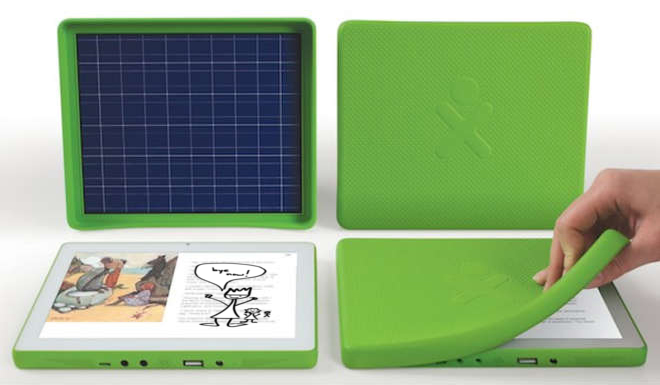
\epsfig{file=xo3-4.eps, width=3.2in}
\caption{Nell's solar-powered hardware platform.  The tablet design
  allows for direct interaction.}\label{fig:xo3}
\end{figure}
% tell a nell story up front
Miles from the nearest school, a young Ethiopian girl named Rahel turns on her
new tablet computer. The solar-powered machine speaks to her:
\textit{``Hello!  Would you like to hear a story?''}

She nods and listens to a story about a princess.  Later, when
the girl has learned a little more, she will tell the machine that the
princess is named ``Rahel'' like she is and that she likes to wear blue---but
for now the green book draws pictures of the unnamed Princess for
her and asks her to trace shapes on the screen.

\textit{``R is for Run.  Can you trace the R?''}

As she traces the R, it comes to life and gallops across the screen.
\textit{``Run starts with R.  Roger the R runs across the Red Rug.
Roger has a dog named Rover.''}  Rover barks: \textit{``Ruff! Ruff!''}  The
Princess asks, \textit{``Can you find something Red?''} and Rahel uses the
camera to photograph a berry on a nearby bush.

\emph{``Good work!  I see a little red \underline{here}.  Can you find
something \underline{big} and red?''}
% avoid excessive/unmerited praise
% try to say *what* you like, rather than just vague praise
% provide quality feedback, encourage the kid to max out the meter on
% their own (ie, making the kid proud of himself for doing well is
% better than telling him they're doing well)

As Rahel grows, the book asks her to trace not just letters, but whole
words.  The book's responses are written on the screen as it speaks
them, and eventually she doesn't need to leave the sound on all the
time.  Soon Rahel can write complete sentences in her special book,
and sometimes the Princess will respond to them.  New stories teach her about
music (she unlocks a dungeon door by playing certain tunes) and
programming with blocks (Princess Rahel helps a not-very-bright turtle
to draw different shapes).  Rahel writes her own stories about the Princess,
which she shares with her friends.  The book tells her that she is
very good at music, and her lessons begin to encourage her to invent
silly songs about what she's learning.

An older Rahel learns that the block language she used to talk with
the turtle is also used to write all the software running inside
her special book.  Rahel uses the blocks to write a new sort of rhythm
game.  Her younger brother has just received his own green book,
and Rahel writes him a story which uses her rhythm game to help him learn
to count.

\section{Key Ideas}
The interaction design of the Nell system described above is inspired
by the ``Young Lady's Illustrated Primer'' in the Neal Stephenson
novel \textit{The Diamond Age}, from whose protagonist Nell takes its
name.\footnote{In a nod to Seymour Papert, Nell can also be read as an
acronym for ``Narrative Environment for Learning Learning.''}
Nell's design embodies four key ideas: it is a \textbf{Narrative}
interface using \textbf{Direct Interaction} which \textbf{Grows} with,
and is \textbf{Personalized} for, the child.
Nell uses these four key concepts to build a novel learning platform
which addresses several challenges we've encountered in earlier work.

%Section~\ref{sec:related} discusses related work.
%The final section will draw conclusions and describe future work.

\subsection{Narrative}
%used to \cite{flores:uruguay,idb:peru} below; removed for space

Children (like all humans) are hard-wired for stories~\cite{boyd:stories}.
In our earlier learning software, we've seen some of our favorite
pedagogical activities neglected because children had difficulty
finding their way into the material without an enthusiastic teacher's
guidance.  In response, Nell uses a
\textit{Narrative Interface}~\cite{bizzocchi:narrative,don:narrative}
to pave a path for the child user through the learning material.
In the narrative interface, all system actions are shaped by a
storybook metaphor, and
interactions with the system are framed as interactions with one of the
system protagonists.

Nell's overall story is a multi-character serial adventure, taking
cues from \textit{The Diamond Age} and
from the UNIVERSE narrative-generation system~\cite{lebowitz:universe85}.
Each of the several characters represents a specific skill or subject
area, and each adventure represents about a year's curriculum.
Adventures are further subdivided into story modules, which match the
scope of a traditional lesson plan.  The serialized multi-character
design improves modularity and allows updates and decentralized
authorship.

%\begin{figure}
%\centering
%
\epsfig{file=roger1.eps, height=1.5in} % width=3.2in
%\caption{Diagram of Nell's primary interface.}\label{fig:nell}
%\end{figure}

%As depicted in Figure~\ref{fig:nell},
Nell's characters are
always-available agents layered above a particular system \textit{activity}
(application) which provides specialized functionality.  The agents
are not always foregrounded: constructionist learning occurs when the
child plays freely to ``make things'' with the base activity.
The handwriting tutor is fundamentally a drawing activity; the
adventure involving the magical musical lock is also a music-making activity.
%  ``Making things'' is the key to constructionist learning.
The narrative system is
hooked into each activity to provide passive guidance
(congratulating the child when it notices they've drawn a letter),
active guidance (Apple-Guide--style~\cite{powers:appleguide}
contextual help), or system services (switching activities; jumping into a
related story module).  A system-wide \textit{achievement} system provides
goals and rewards.

% Story Module == Lesson Plan

% not always a story -- kid can draw on their own and return to the
% story; Nell will observe the free play and offer suggestions.
\subsection{Personalized}
% customization, renaming characters

% MSTONE FEEDBACK: lead off w/ responding to learning styles, not
% changing colors.  (Also incorporate learning style stuff into
% section 1.)  Move color changing into Related Work, even?

Children learn in different ways.  Nell provides multiple
story modules for its plot points/lessons to engage the child's
interests and cater to multiple intelligences~\cite{gardner:mi}.
Selecting between the alternatives can depend on either explicit
choices made by the child (``fractions in outer space,'' if the child
chose a space-themed story or previously indicated an interest in space)
or prior success with a given
lesson style (a large number of accomplishments in musical-rhythmic
tasks suggests a rhythmic approach to fractions).  Similarly, several
different achievements can coexist, rewarding different ways of
accomplishing the same pedagogical goal.

The record of past choices and accomplishments is stored in a
\textit{Journal} and can be reviewed by the child.  The contents of the
Journal can be rearranged to create a Portfolio~\cite{stefanakis:portfolios}
demonstrating the child's progress.
In order to encourage fearless play and experimentation, the Journal
also supports pervasive undo; the child can rewind and replay the
narrative starting at any past point in the journal.

Content can be remixed for further personalization.
The child is encouraged to rename characters and change clothing,
colors, and other superficial details.  In the future
we expect to accomplish further narrative customization by
recombination of story elements.
Lebowitz~\cite{lebowitz:universe85} and Riedl~\cite{riedl:planning}
show how a planner can be used to recombine and adapt story fragments.
We have less ambition than the cited work: instead of
attempting to generate thousands of stories from tens of templates, we
hope to select and then modestly adapt from hundreds of story
modules created in a decentralized manner by teachers---and eventually
by the students themselves.

\subsection{Growable}

% MSTONE FEEDBACK: 'accumulating' in 3rd sentence starts conflating
% serial 'tech tree' of story material w/ 'decentralized authoring'
% mechanism of expanding topics covered by the system.
% Move 'tech tree' aspect to personalization: ``ie, not only does
% the system personalize based on learning style, but also based
% on achievement''.  last paragraph can segue into 'growable'
% which is mostly about 3rd party expansion.

% CSA: three axes of growth
%  1. serial tech tree of story material; more advanced topics
%  2. turtlescript -- metacircular understanding of the system itself
%  3. community -- no limit to content creation, including by the child.

Children grow.  Nell aims to provide a ``low floor and no ceiling'' to
grow with them, along three main axes.
%There are three main axes of growth.
%  Nell's low floor is its
%simple base system,
%usable with no literacy skills or external guidance.
%From there Nell grows in three directions.

First, Nell tracks the child's growing intelligence and capability
with increasingly challenging story material.  As the child
accumulates achievements and demonstrates
proficiency, the serial story moves on to more advanced topics.

Second, Nell seeks to grow its authoring community.  Decentralized
authorship ensures that Nell's instructional content
continues to increase in the number of topics and
customizations.  There are no
ceilings between children and teachers: Nell
contains a story editor and everything necessary to
author and publish story modules.

To further promote collaboration,
Nell is free and open source and implemented in standard web
technologies (JavaScript, HTML5, and WebGL) with offline caching.
Resources are named by URL, even when disconnected from the
internet, which simplifies the distribution of updates to story modules and
the Nell system.  URL-based identifiers also allow third parties
to manage their own namespaces when extending Nell.

Finally, Nell is designed to allow a capable child to learn about
the construction of the system itself,
eliminating the ceiling between the child and
the authors of the Nell system.  Nell can teach
about itself, and its source code is open for exploration within Nell.
Meaningful changes can be performed without external tools.

%.  Meaningful changes to the Nell system can
%be performed on the system itself.
%In Section~\ref{sec:turtles} we describe how this goal is approached.

%As far as possible, Nell is implemented in JavaScript.
% if the kid's going to learn some software stack, this seem like a
% fine one to learn


% it has a ``low floor and no ceiling'' to allow a child to master more
% and more of the system as she grows.
% modular -- the story expands.
% text read aloud initially

\subsection{Direct interaction}
% constructionist?
% handwriting as UI?
% motor skills
% photo of XO-3?

%MSTONE PARALLEL STRUCTURE:
%Children often learn from direct interactive experience. Consequently, Nell
%intensifies our commitment to constructionism~\cite{Papert91} by further
%emphasizing creation and tangible interaction using a tablet computer as a way
%to maintain the child's connection to their work (Fig.~\ref{fig:xo3}).

The constructionist learning philosophy emphasizes creation and
tangible interaction.  Nell uses direct interaction on a tablet
computer to maintain the child's connection to their work
(Figure~\ref{fig:xo3}).  In particular, Nell uses handwriting
recognition as a primary interface.

The direct interaction model lowers the floor by eliminating the need
to learn an abstract touchpad or mouse interface.  It also supports
our literacy goals by allowing direct handwriting instruction and
development of motor skills.

\section{Technology}
%Our technology choices further our goals of modularity and
%decentralization.  Nell's implementation is free and open source and uses
%standard web technologies to broaden the contributor base.  In this
%section we describe the technologies that enable Nell's four key ideas.

Our implementation choices further our goals of modularity and
decentralization.  In this
section we describe the technologies that enable Nell's four key ideas.

\subsection{Rule-based story modules}
\begin{figure}\small
\begin{verbatim}
{ "world": { // id gives canonical URL for this module
    "id": "/nell.laptop.org/chapters/alphabet-book",
    "scene": "opening", // initial scene
    "inherit_from": "/nell.laptop.org/core/drawing_activity",
  }, "scenes": [
    { "id": "opening", subject: "actors/princess",
      "verb": "speak", object: "actors/user",
      "text": "Hello! Would (o/2) like to hear a story?",
      "group": "/nell.laptop.org/core/story-intro-group",
    },
    { "id": "story-1",
      "cond": rule`At(opening) && Event(Chat, Yes)`,
      "subject": "actors/princess",
      "verb": "speak", object: "actors/user",
      "text": "Once upon a time..." },
    ...
    { "id": "r-drawn",
      "cond": rule`Event(Activity, DrawR)`,
      "subject": "actors/princess",
      "verb": "speak", object: "actors/user",
      "text": "Very good, (o/3)!",
      "action": js`startAnimation("r-runs")` }, ...
  ], ... }
\end{verbatim}
\caption{Story module excerpt written in JSON
  (\texttt{http://json.org}) extended with
 quasiquote~\cite{quasiquote}.}\label{fig:rules}
\end{figure}
To implement Nell's modular narrative interface, we use a
production rule system with programmable conflict resolution.
Figure~\ref{fig:rules} shows
an excerpt of the story module underlying the interaction described in
Section~\ref{sec:lesson}.

Stories consist of a sequence of \textit{scenes} plus information about
characters, locations, and activities.  Scenes are ``goals''
in the STRIPS formalism~\cite{strips} and consist of
action descriptions, preconditions, and effects.
In principle, all preconditions for all scenes of all story modules
are evaluated continuously to determine the actions of the narrative
agents.  This evaluation
is made computationally efficient using the Rete
algorithm.  Dialog is expressed using Curveship-style
templates, allowing Nell to restructure
expository tense, style, and point-of-view~\cite{montfort:curveship}.

%  The Rete algorithm requires that our conditions are in Normal
%  Form\footnote{BE PRECISE HERE}, but actions can be arbitrarily complex.

New story modules can be downloaded from the Internet in
connected deployments.  In disconnected deployments, new stories
might be distributed once a year on USB sticks or shared among
friends.  In a classroom environment, a teacher can share stories for
the day's lesson at the start of class.

Story modules can be inherited and extended.
This makes it easy to take an existing story and modify it to
better suit particular interests, a particular type of learner---or
just to add variety.  This can lead to conflicts: multiple versions of
a story, or scenes within a story, may have their
preconditions satisfied simultaneously.

Conflicts are resolved by consulting a \textit{group} associated with
each scene.  Each group has a default priority and names a scene to be
invoked when a conflict exists; the actions associated with that scene
will (eventually) alter the priorities of the conflicting scenes to
resolve the conflict.  The resolution scene may include any number of
actions.  It may select randomly among the conflicting scenes or base
its selection on the
child's preferences, curriculum progress, or inferred learning style.
The resolution scene may even initiate a new multi-scene story.

For example, the \textit{story-intro-group}
used in Figure~\ref{fig:rules} defaults to a low priority so that
continuing a story in progress is preferred above starting a new story.
When a story module is completed, several new story openings will be in
conflict.  The resolution scene for \textit{story-intro-group} may bring us
to the controls of an airship which flies between locations
corresponding to the various story continuations.  In that set of
scenes, the child may eventually decide to fly to Mathland to hear the
next episode in her agent Mathis' adventure, which would bump up the
appropriate scene's priority to make the transition
without further conflict.

Nell will include an integrated story editor.  Our exemplar is
the Wide Ruled authoring tool, which was successfully used by
non-technical story creators~\cite{skorupski:2009}.

% excerpt of story model
% rete algorithm, cite Riedl, etc.
% programmable conflict resolution
% cite the story editor from Wide Ruled

\subsection{Extensible dialog}
Nell's use as an interactive diary and
\textit{portfolio}~\cite{stefanakis:portfolios} is enhanced by the child's
collaboration in the fiction that Nell is intelligent---what
Turkle~\cite{turkle:alone} calls the ``ELIZA effect.''
Convincing discourse is a hard problem, but
reasonable approximations do not have to be difficult; even
the rudimentary conversational abilities of ELIZA elicited hours of
conversation.%~\cite{weizenbaum:power}
% her secretary is divulging her life story
% asks him to leave the room so he could be alone with it
% hours discussing her boyfriend.
We've chosen to allow the child to directly converse with the
Princess and other agents within Nell.

\begin{figure}\small
% (could remove
%  "version": "1.0",
% before "categories" in order to save space in paper)
\begin{verbatim}
{ "aiml": {
  "version": "1.0",
  "categories": [
    { "pattern": "GO *",
      "template": "{*}" },
    { "pattern": "N",
      "template": "{NORTH}" },
    { "pattern": "NORTH",
      "template": js`FireEvent(Chat, "NORTH")` },
    { "pattern": "* THE DOOR",
      "template": "{*} DOOR" },
    { "pattern": "* SQUEAKY DOOR",
      "template": "{*} DOOR" },
    { "pattern": "OPEN DOOR",
      "template": js`FireEvent(Chat, "OPEN DOOR")` }
  ] } }
\end{verbatim}
% alternate template syntax, compatible w/ quasiquote but not
% dependent on it:
% template: "${srai(star(0))}" // can be abbreviated as srai(star()) or srai()
% template: "${srai("NORTH"}}"
% template: "${FireEvent(Chat, "NORTH")}"
% template: "${srai()} DOOR" // abbreviation for srai(star(0))
\caption{An AIML fragment which recognizes the commands
  %\texttt{N},
  \texttt{North}, \texttt{Go North}, \texttt{Open the squeaky door}
  and variants.  AIML's XML syntax has been translated to JSON.
  Template contents in braces invoke the recognizer recursively
  (what AIML calls \texttt{<srai>}).
% XXX: how to handle multiple stars?  In XML, it's <star index="1">
}\label{fig:aiml}
\end{figure}

Our implementation extends AIML~\cite{aiml:2005},
the markup language developed for the Loebner Prize--winning
AliceBot.%
\footnote{Wilcox identifies several shortcomings with the expressive
  power of AIML, proposing ChatScript as a
  replacement~\cite{wilcox:2010}.  AIML's community and
  diversity of third-party implementations make it our choice at present.}
Each story module can include AIML fragments extending the
conversational capabilities of Nell's agents.
% we say this in the figure, don't repeat it here? ==>
%    We have translated AIML's XML-based syntax to JSON.

Figure~\ref{fig:aiml}
shows an AIML fragment augmenting an agent with
commands suitable for a text adventure story module.
In such a story the child might write instructions such as
\texttt{go north}, \texttt{go east}, or \texttt{open door} in
addition to the usual dialog with the agent.
These new commands fire events which are referenced by scene
preconditions.  For example, \texttt{north} may
trigger a scene which causes the activity to draw a new location on
the page, causes the agent to write and speak a description of the new
location, and finally causes a shift in the AIML \textit{topic} to
enable additional vocabulary suitable for the new location.

% xx can the activity influence which commands are active?
% yes, by shifting the topic.  AIML should have a more flexible
% topic system.

\subsection{TurtleScript}\label{sec:turtles}

We have developed a block-oriented view of JavaScript, which we call
TurtleScript~\cite{turtlescript}.
The TurtleScript dialect of JavaScript is the single
implementation language for Nell.%
\footnote{Since JSON is the data-oriented subset of JavaScript,
our examples in Figures~\ref{fig:rules} and \ref{fig:aiml} are valid
TurtleScript.} % XXX: use TurtleScript tiles for the figures?
TurtleScript scales from Logo-like
pedagogical tasks (in subsets of the language) up to the
implementation of TurtleScript and the
Nell system itself.  As Figure~\ref{fig:turtlescript} shows,
TurtleScript's block view is isomorphic to
JavaScript's standard textual
representation to
% CSA: hard to state all the reasons in just one short phrase, sigh.
ensure the readability of and compatibility with existing JavaScript libraries.
%preserve the code-reading skills of existing programmers.
%
We have begun implementation of a
tablet programming environment for TurtleScript which uses
drag-and-drop, direct interaction, and intelligent prompting to reduce
text entry requirements.

% XXX refer to TurtleScript excerpt in figure somewhere here.
\begin{figure}
\centering
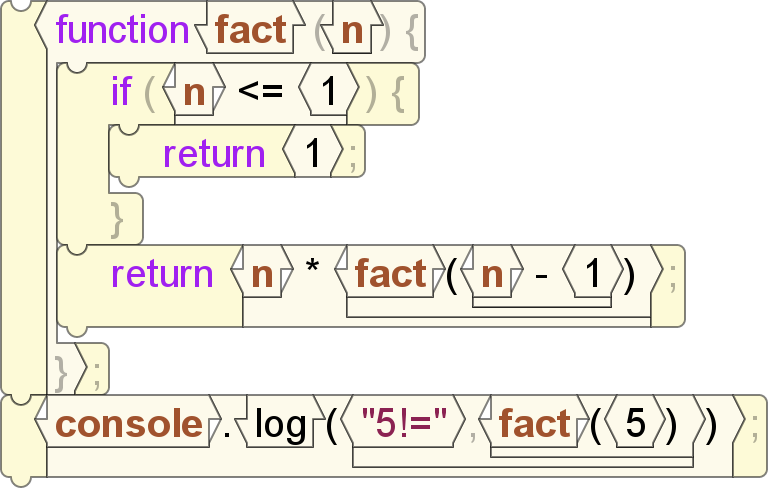
\epsfig{file=turtlescript-2.eps, height=1.3in}
\caption{Factorial function in TurtleScript.}\label{fig:turtlescript}
\end{figure}

TurtleScript allows the child to dig as far into Nell's implementation
as their capabilities allow.  Although the operating system and the
browser implementation remain inaccessible, incorporating a
meta-circular interpreter for JavaScript%
\footnote{For example, \url{https://github.com/mozilla/narcissus/}}
% (such as \cite{narcissus})
allows us to expose the system all the way down to the programming
language implementation.
% Via TurtleScript, this code is all visible in a
% friendly block-based form.

% Javascript/HTML5
% offline caching
% turtles (almost) all the way down (turtlescript again)
% excerpt of TurtleScript

\section{Related work}\label{sec:related}

The TinkRBook system~\cite{chang:tinkrbook} shares a similar focus on
personalization and literacy.  Nell attempts to scale the system up
with a modular extensible narrative system and a broader range
of pedagogic material.

The Sugar Learning Platform~\cite{sugar} is an earlier effort at
child education in which we've been directly involved.  Nell's focus is
on children further from educational infrastructure than those
targeted by Sugar.
The narrative at Nell's core attempts to provide students
pedagogical guidance missing from Sugar,
and the direct interaction model avoids keyboard
problems which have plagued Sugar's initial deployments.  Nell also
attempts to provide a greater sense of ownership through pervasive
customization.

% MSTONE FEEDBACK: ``the innovations vis-a-vis Sugar are: a) authoring
% and publishing is a first-class concept, instead of just
% "synchronous collaboration" and b) there's a pedagogically motivated
% feedback loop; it's not just an open-loop "constructionist" system''

% MSTONE TEXT
% Nell takes advantage of this fact 
% to augment prior affordances for \textit{action}, \textit{reflection}, and
% \textit{communication} with new affordances for \textit{engagement} in the form of
% a modular \textit{Narrative Interface}~\cite{bizzocchi:narrative,don:narrative}.

Automatic narrative generation has seen attention in
gaming, simulation, and training contexts~\cite{riedl:2008}.
We believe
Nell's synthesis of these ideas in a pedagogical context is unique.

\section{Conclusions}
We have described the design of a novel narrative direct-interface
system for education, beginning with literacy, which is personalized for and grows with
its child owner.  Personalized direct interface engages the child, and
narrative guides them through pedagogic material.  Low-cost
solar-powered hardware allows Nell to reach further into the
least-developed areas of the world to help those without traditional
educational infrastructure.

We are in the process of implementing the Nell system, and expect to
field initial deployments of subsets of Nell in Africa later this year.
Volunteer assistance is welcome.

% CSA: Acknowledge the below in the related work, rather than spending
% space on a heading and a new section.

%% \section{Acknowledgments}
%% Nell's design evolved from experience with the Sugar system,
%% architected by Walter Bender, and through stimulating discussions with
%% the Sugar community and Angela Chang.

%
% The following two commands are all you need in the
% initial runs of your .tex file to
% produce the bibliography for the citations in your paper.
\bibliographystyle{abbrv}

% ACM needs 'a single self-contained file'!
%\bibliography{paper}  % paper.bib is the name of the Bibliography in this case
\begin{thebibliography}{10}

\bibitem{aiml:2005}
{A.L.I.C.E. AI Foundation}.
\newblock Artificial intelligence markup language ({AIML}) version 1.0.1.
\newblock \url{http://www.alicebot.org/TR/2005/WD-aiml/}, 2005.

\bibitem{turtlescript}
C.~S. Ananian.
\newblock \url{http://cscott.net/Projects/TurtleScript/}, 2011.

\bibitem{bizzocchi:narrative}
J.~Bizzocchi.
\newblock Games and narrative: An analytical framework.
\newblock {\em Loading---the Journal of the Canadian Games Studies
  Association}, 1(1), 2007.

\bibitem{boyd:stories}
B.~Boyd.
\newblock {\em On the Origin of Stories: Evolution, Cognition, and Fiction}.
\newblock Belknap Press of Harvard University Press, 2009.

\bibitem{chang:tinkrbook}
A.~Chang and C.~Breazeal.
\newblock {TinkRBook}: Shared reading interfaces for storytelling.
\newblock In {\em Proc. of the 10th Int'l Conf. on Interaction Design and
  Children (IDC '11)}, pages 145--148. ACM, June 2011.

\bibitem{don:narrative}
A.~Don.
\newblock Narrative and the interface.
\newblock In B.~Laurel, editor, {\em The Art of Human-Computer Interface
  Design}, pages 383--391. Addison-Wesley, Reading, MA, 1990.

\bibitem{strips}
R.~E. Fikes and N.~J. Nilsson.
\newblock {STRIPS}: A new approach to the application of theorem proving to
  problem solving.
\newblock {\em Artificial Intelligence}, 2(3--4):189--208, 1971.

\bibitem{gardner:mi}
H.~E. Gardner.
\newblock {\em Frames Of Mind: The Theory of Multiple Intelligences}.
\newblock Basic Books, Dec. 1983.

\bibitem{lebowitz:universe85}
M.~Lebowitz.
\newblock Story-telling as planning and learning.
\newblock {\em Poetics}, 14(6):483--502, Dec. 1985.

\bibitem{montfort:curveship}
N.~Montfort.
\newblock Curveship's automatic narrative variation.
\newblock In {\em Proc. of the 6th Int'l Conf. on the Foundations of Digital
  Games (FDG '11)}, pages 211--218, June 2011.

\bibitem{powers:appleguide}
J.~Powers.
\newblock Giving users help with {A}pple {G}uide.
\newblock {\em develop}, 18, June 1994.
\newblock Apple Computer, Inc.

\bibitem{riedl:2008}
M.~O. Riedl, A.~Stern, D.~Dini, and J.~Alderman.
\newblock Dynamic experience management in virtual worlds for entertainment,
  education, and training.
\newblock {\em Int'l Trans. on Systems Science and Applications}, 3(1), 2008.

\bibitem{riedl:planning}
M.~O. Riedl and R.~M. Young.
\newblock Narrative planning: Balancing plot and character.
\newblock {\em Journal of Artificial Intelligence Research}, 39:217--267, 2010.

\bibitem{quasiquote}
M.~Samuel.
\newblock Ecmascript quasi-literals.
\newblock \url{http://wiki.ecmascript.org/doku.php?id=harmony:quasis}, 2012.

\bibitem{skorupski:2009}
J.~Skorupski and M.~Mateas.
\newblock Interactive story generation for writers: Lessons learned from the
  {W}ide {R}uled authoring tool.
\newblock In {\em Proc. of the 8th Digital Art and Culture Conf. (DAC)},
  Irvine, CA, Dec. 2009.

\bibitem{stefanakis:portfolios}
E.~Stefanakis.
\newblock {\em Multiple Intelligences and Portfolios: A Window Into The
  Learner's Mind}.
\newblock Heinemann, 2002.

\bibitem{sugar}
{Sugar Labs}.
\newblock \url{http://sugarlabs.org}.

\bibitem{turkle:alone}
S.~Turkle.
\newblock {\em Alone Together: Why We Expect More From Technology and Less From
  Each Other}.
\newblock Basic Books, 2011.

\bibitem{wilcox:2010}
B.~Wilcox.
\newblock Beyond {F}a\c{c}ade: Pattern matching for natural language
  applications.
\newblock
  \url{http://chatscript.sourceforge.net/Documentation/Pattern_Matching_for_Natural_Language_Applications.pdf},
  Feb. 2011.

\end{thebibliography}

%
%\balancecolumns
% That's all folks!
\end{document}

%%  LocalWords:  personalization Lebowitz TurtleScript AIML Loebner
%%  LocalWords:  AliceBot modularity Rahel Ananian Akamai Papert JSON
%%  LocalWords:  Riedl WebGL touchpad Curveship Rete TinkRBook
